\sectionframe{Kurz\-ein\-füh\-rung in die Gra\-phen\-the\-orie}

\begin{frame}
 \frametitle{Beispiel: Lewig Adelburg}
 \begin{figure}
  \centering
  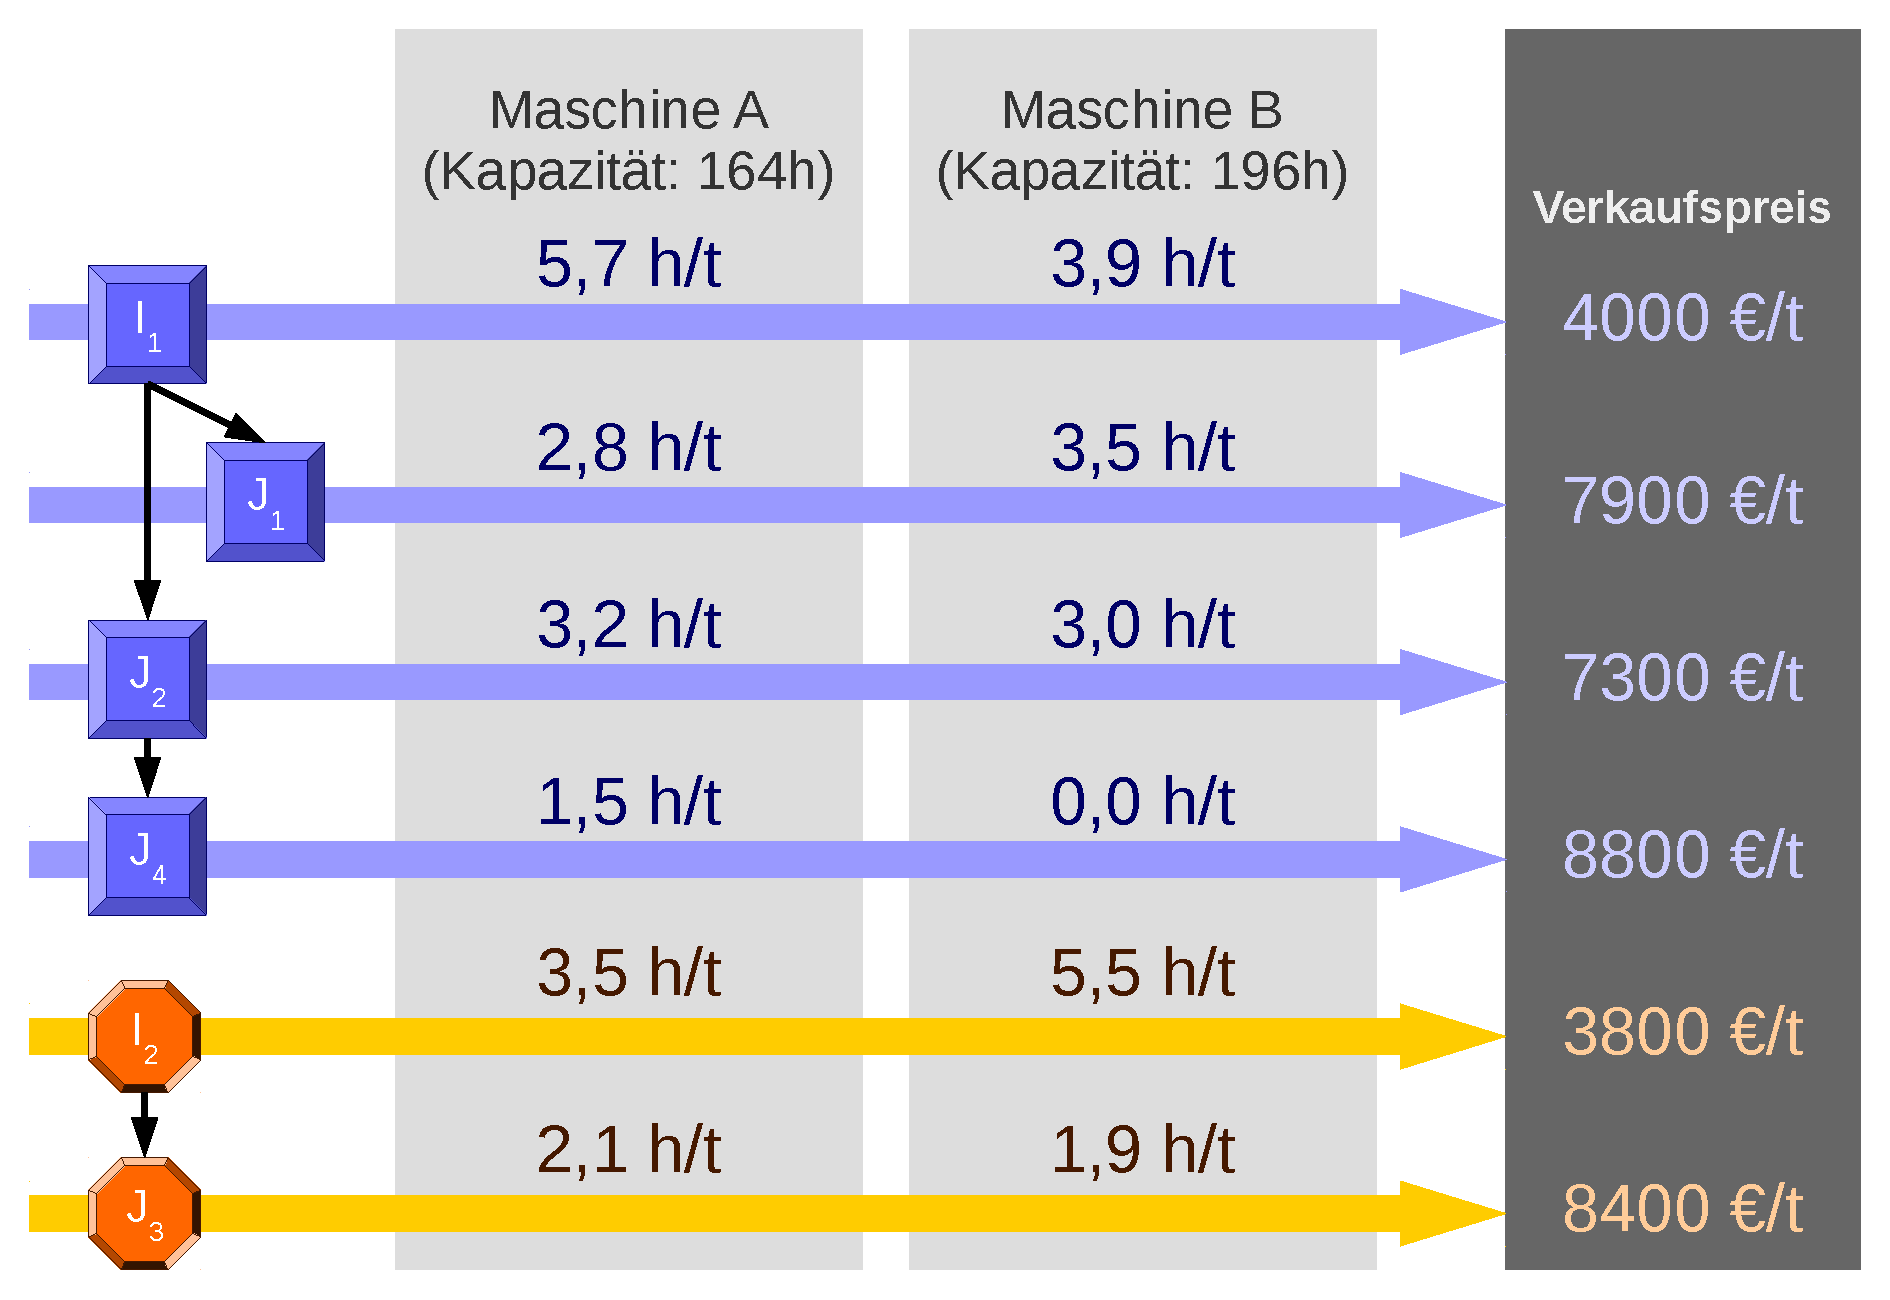
\includegraphics[width=\linewidth]{Bilder/LewigAdelburg}
 \end{figure}
\end{frame}

\begin{frame}
 \frametitle{Graphenbegriff: Komponenten}
 \begin{center}
  \includegraphics<1>[width=.7\linewidth,page=1]{Bilder/Graph_Lewig_Adelburg}
  \includegraphics<2>[width=.7\linewidth,page=2]{Bilder/Graph_Lewig_Adelburg}
 \end{center}
\end{frame}

\begin{frame}
 \frametitle{Graphenbegriff: Formale Beschreibung}
 \begin{itemize}
  \item \textbf{Gerichtete} Graphen sind definiert als ein Tupel $G=(V, E)$ mit einer Knotenmenge~$V$ und einer Kantenmenge~$E\subseteq V\times V$.\\[1ex]
    Im Beispiel:\\{\footnotesize $G = (\{I_1, I_2, J_1, J_2, J_3, J_4\}, \{(I_1, J_1), (I_1, J_2), (I_2, J_3), (J_2, J_4)\})$}
  \item \textbf{Ungerichtete} Graphen sind Graphen, deren Kanten keine feste Richtung haben.
  \item \textbf{Gewichtete} Graphen sind definiert als ein Tupel $G=(V, E, g)$ mit einer Knotenmenge~$V$, einer Kantenmenge~$E\subseteq V\times V$ und einer Gewichtungsfunktion $g:E\rightarrow\mathbb{R}$.
 \end{itemize}
\end{frame}
